\documentclass[tikz,border=2pt]{standalone}
\usepackage{pgfplots}
\pgfplotsset{compat=1.18}
\begin{document}
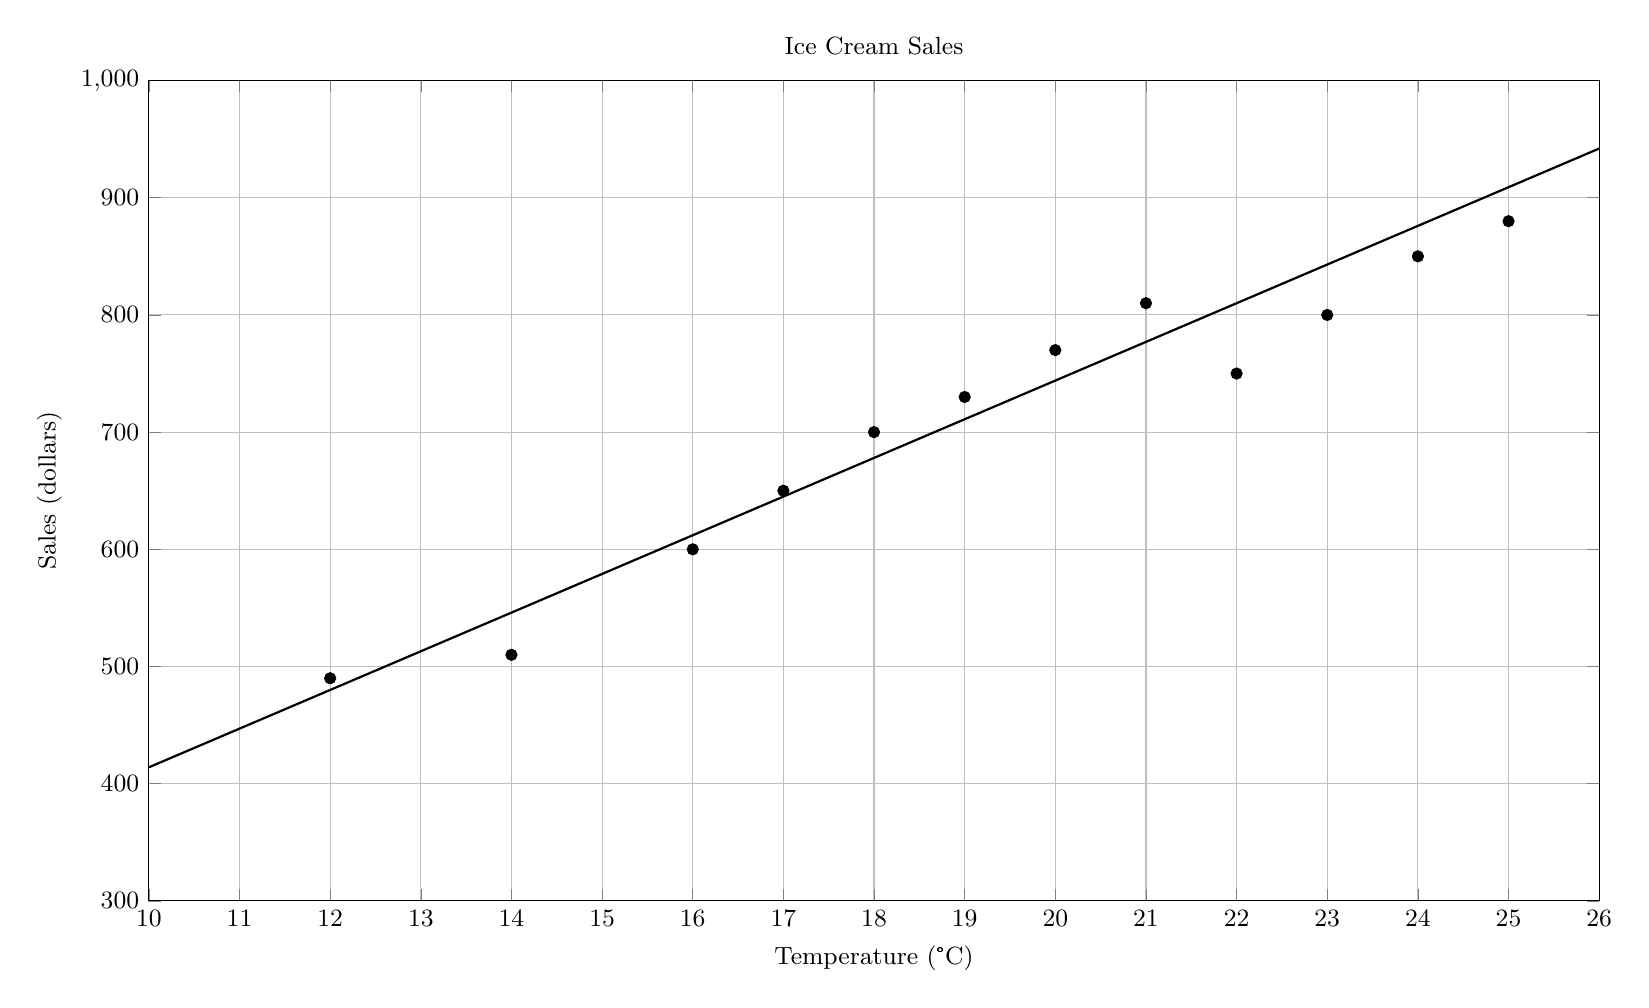
\begin{tikzpicture}
\begin{axis}[
    xlabel={Temperature (°C)},
    ylabel={Sales (dollars)},
    ytick={300,400,...,1000},
    xmin=10, xmax=26,
    ymin=300, ymax=1000,
    grid=major,
    width=20cm, height=12cm,
    title={Ice Cream Sales},
    font=\small
]
\addplot[
    only marks,
    mark=*,
]
coordinates {
    (12, 490)
    (14, 510)
    (16, 600)
    (17, 650)
    (18, 700)
    (19, 730)
    (20, 770)
    (21, 810)
    (22, 750)
    (23, 800)
    (24, 850)
    (25, 880)
};
\addplot[domain=10:26, thick] {33*x + 84};
\end{axis}
\end{tikzpicture}
\end{document}
